\chapter{Antenne patch o a microstriscia}
Le antenne patch sono antenne planari, che possono essere quindi stampate o incise su ogni genere di supporti rigidi.

Esse, quindi, sono spesso utilizzate nei circuiti integrati e trovano ampia applicazione nei dispositivi mobili, dove lo spazio occupato è di grande importanza e dove antenne ad ampio raggio sono preferite rispetto a quelle più direttive.

L'antenna patch più semplice è un antenna rettangolare, come in \autoref{fig:patch}.

\begin{figure}[htp]
	\centering
	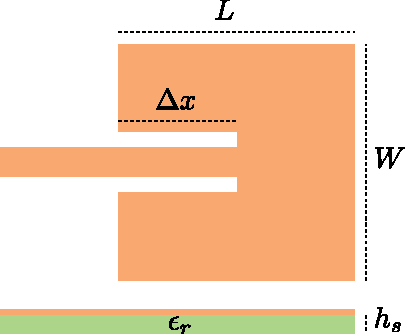
\includegraphics[]{img/patch.pdf}
	\caption{Visione dall'alto e dal lato dell'antenna patch. Le parti in arancione sono di \gls{pec}, mentre il substrato verde è composto da un materiale dielettrico.}
	\label{fig:patch}
\end{figure}

\section{Parametri d'antenna}

Attraverso le dimensioni dell'antenna e il tipo di materiale dielettrico si può regolare la frequenza di risonanza, mentre il parametro $\Delta x$ di lunghezza dell'\emph{inset} regola l'impedenza dell'antenna.

Prima di tutto si calcola la larghezza dell'antenna, partendo dalla lunghezza d'onda desiderata.

\begin{equation*}
	W =\frac{\lambda}{2 \sqrt{\frac{\epsilon_r+1}{2}}}
\end{equation*}

Definiamo ora la \emph{costante dielettrica efficace} dell'isolante, che impiegheremo nel calcolo della lunghezza della patch e della larghezza di banda $B\%$.

\begin{esp}\label{eq:paramPatch}
	\epsilon_{re}
	&= \frac{\epsilon_r+1}{2} +\frac{\epsilon_r-1}{2}\sqrt{1+\frac{10 h_s}{W}} \\
	L&=\frac{\lambda}{2\sqrt{\epsilon_r}}
	- \frac{\left(\epsilon_{re} +0.3 \right) \, \left(\frac{W}{h_s}
	+ 0.264\right)}{\left(\epsilon_{re} +0.258 \right)\, \left(\frac{W}{h_s} + 0.8\right)} \\
	&\simeq 0.49 \, \frac{\lambda}{\sqrt{\epsilon_r}} \\
	B_\%&= 3.77 \, \frac{\epsilon_r-1}{\epsilon_r^2} \, \frac{W}{L}\, \frac{h_s}{\lambda}
\end{esp}

L'impedenza d'antenna risulta quindi, non creando un inset al suo interno,
\begin{equation}\label{eq:ZaPatch}
	Z_A(\Delta x=0)
	= 90 \frac{\epsilon_r^2}{\epsilon_r-1} \left(\frac{L}{W}\right)^2
\end{equation}

Nel caso in cui si inserisca l'inset, è sufficiente modificare la formula appena ricavata, in questo modo.
\begin{esp}
	Z_A(\Delta x)
	%&=Z_A(\Delta x=0) \, \cos^2 \left(\pi \, \frac{\Delta x}{L} \right) % questa formula (del libro) è sbagliata, diceva il Santa
	&= Z_A(\Delta x=0) \, \cos^4 \left(\pi \, \frac{\Delta x}{L} \right)
\end{esp}

Inoltre, in una patch con inset, l'asse centrale (a $W / 2$) dell'antenna ha campo nullo, per cui è possibile inserire qui un piano di massa, dimezzando le dimensioni dell'antenna.

\subsection{Qualità dell'antenna}
Definiamo qualità dell'antenna il rapporto tra energia elettromagnetica $W$ e potenza irradiata $P$ a una certa frequenza $f$, ossia
\begin{equation}
	Q_A=2\pi f \frac{W}{P} \ge \frac{1}{(\beta D)^3}
\end{equation}
dove $\beta = \frac{2\pi}{\lambda}$ e $D$ è la dimensione dell'antenna.

Come si può notare, la qualità presenta un limite superiore: non è possibile quindi, neppure con gli apparecchi più sofisticati, ottenere un'efficienza d'antenna arbitraria.

\section{Bilanciamento antenne e BAL-UN}

Spesso le antenne reali presentano delle asimmetrie, dovute alla fabbricazione oppure all'interferenza con i cavi di alimentazione.

Per questo è opportuno, per \emph{bilanciare questi sbilanciamenti} (BALance-UNbalanced) cortocircuitare tra loro elementi dell'antenna.

Per esempio, nel caso di asimmetria tra i due bracci del dipolo a mezz'onda, è possibile cortocircuitare una parte della sezione più lunga per correggere questa differenza di lunghezza.

%%% Local Variables:
%%% mode: latex
%%% TeX-master: "antenne"
%%% End:
